\section{Inferencia de tipos} % (fold)
\label{sec:inferencia_de_tipos}

% section inferencia_de_tipos (end)

Haskell permite definir funciones sin decir de que tipos son estas, esto, muy lejos de querer decir que Haskell no usa un tipado fuerte, es debido a que realiza inferencia de tipos.
Uno puede escribir una función que sume dos números como:

\begin{lstlisting}
  sumar  ::  (Num a) => a -> a -> a
  sumar x y = x + y
\end{lstlisting}

Donde la primer linea indica que las variables \textbf{a} son de la clase de tipos \textit{Num}.
Si en GHCI usamos el comando \textbf{:t} para pedir el tipo de la funcion sumar tendremos:

\begin{lstlisting}
  :t sumar
  sumar  ::  (Num a) => a -> a -> a
\end{lstlisting}

Este resultado era evidente, ya que en la propia definición lo habíamos indicado. Pero Haskell permite definir la función sumar de la siguiente manera:

\begin{lstlisting}
  sumar x y = x + y
\end{lstlisting}

Al utilizar el comando :t en GHCI obtendremos la misma respuesta que antes, aunque esta vez no le  hayamos indicado al lenguaje los tipos en la definición.

\subsection{Algoritmo de Hindley-Milner} % (fold)

% subsection algoritmo_de_hindley_milner (end)
Este resultado proviene de que Haskell realiza inferencia de tipos basandose en el algoritmo de Hindley Milner o Damas Milner.
Este algoritmo sigue seis reglas lógicas:
\begin{figure}[H]
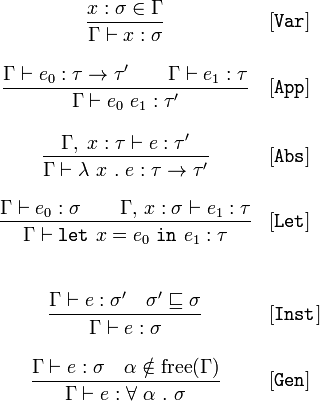
\includegraphics[width=80mm]{hindley-milner}
\end{figure}

Para explicar que quieren decir estas seis reglas primer es necesario entender la sintaxis y el significado de alguno de los símbolos.

Lo primero es la barra horizontal, esta viene a cumplir el rol de una implicación lógica, o sea, si el antecedente, lo de arriba, es verdadero entonces, necesariamente, el consecuente, lo de abajo, también lo es. Cuando en la parte superior hay N hipótesis, para asegurar el consecuente es necesario que se cumplan las N hipótesis, es como si las separaciones por espacio estubiesen indicando una operación and lógica.
Lo siguiente son los dos puntos \lstinline$":"$, estos indican de que tipo es una expresión, por ejemplo x : Int indica que x es del tipo int. El contexto se representa con $\gamma$. Para indicar que algo se encuentra en un determinado contexto usamos $\in$. $\vdash$ es básicamente que se puede demostrar algo, lo precede el contexto necesario para demostrar lo que quiere. La coma \lstinline$","$ es utilizada para ampliar el contexto, una unión, si entendemos al contexto como el conjunto de referencias a variables de determinados tipos, donde se pisa el elemento si este ya se encontraba en el contexto original. Por ultimo, el símbolo $\sqsubseteq$ indica una especie de inclusión, en realidad es mas bien una herencia, donde el tipo de la izquierda es un subtipo del de la derecha.
Con todos la notación clara es sencillo entender las seis reglas.
Por Ejemplo, la segunda indica que si en nuestro contexto tenemos una expresión e0 que  toma un elemento del tipo  $\tau$ y devuelve otro que es del tipo $\tau$', y en ese mismo entorno tenemos una segunda expresión que es del tipo $\tau$, entonces podemos decir que en ese mismo entorno que la expresión e0 e1 es del tipo $\tau$'.
La quinta nos dice que si en un entorno la expresión e es del tipo $\sigma$' y que $\sigma$' es un subtipo de $\sigma$ entonces la expresión e es del tipo  $\sigma$.

El algoritmo de inferencia de tipos usa estas reglas de forma recursiva. Realiza un ajuste de patrones, donde mira la expresión que tiene, y en cual de los consecuentes encaja mejor, una vez encontrado va a los antecedentes y mira que necesita para que estos se cumplen, si con la información actual es suficiente entonces ha terminado de inducir los tipos, en caso contrario toma estos antecedentes que aun no tiene determinados y vuelve a realizar el mismo ajuste de patrón, y así va infiriendo en cada sub-expresión los tipos necesarios. Cuando encuentra que la información alcanzada es suficiente para cumplir TODAS las hipótesis la inferencia esta completa.

\label{sub:algoritmo_de_hindley_milner}

\subsection{Ejemplo de aplicación del algoritmo} % (fold)
\label{sub:ejemplo_de_aplicaci_n_del_algoritmo}

Si hacemos el seguimiento del como funciona este algoritmo en la función sumar que tenemos más arriba, y utilizando la currificación de Haskell tenemos que la función es de la forma

\begin{lstlisting}
  sumar x y = x + y
\end{lstlisting}

que es lo mismo que

\begin{lstlisting}
  sumar x y = (+) x y
\end{lstlisting}

para ajustar el patrón tomamos

\begin{lstlisting}
  e0 = (+) x
  e1 = y
\end{lstlisting}

esto encaja en el segundo patrón, donde se realiza e0 e1 que es del tipo $\tau$', para esto se induce que e0 es del tipo $\tau$ $\rightarrow$ $\tau$' y que e1 es tipo $\tau$'. Hasta ahora solo sabemos que y es del tipo $\tau$.
Luego hay que ajustar el patrón e0. Donde volvemos a caer en el segundo caso. Entonces tenemos que :

\begin{lstlisting}
  e'0 = (+)
  e'1 = x
\end{lstlisting}

Con e'0 e'1 es del tipo $\tau$ $\rightarrow$ $\tau$'
Concluimos que, dado que e'0 es del tipo $\tau$1 $\rightarrow$ t1' y que e'1 es del tipo $\tau$1, como e'0 e'1 = e0
entonces e0 : $\tau$'1 = $\tau$ $\rightarrow$  $\tau$'
Hasta aquí tenemos que


\begin{lstlisting}[mathescape]
y : $\tau$
x : $\tau$1
(+) :  $\tau$1 $\rightarrow$  $\tau$ $\rightarrow$  $\tau$'
\end{lstlisting}

Además, como (+) : (Num a) => a $\rightarrow$ a $\rightarrow$ a
Por la primera regla tenemos que $\tau$1 $\rightarrow$  $\tau$ $\rightarrow$  $\tau$' = a $\rightarrow$ a $\rightarrow$ a
O sea

\begin{lstlisting}[mathescape]
$\tau$1 = a
$\tau$ = a
t' = a
\end{lstlisting}

Y, finalmente, usando la quinta regla tenemos que

\begin{lstlisting}[mathescape]
$\tau$1 $\sqsubseteq$ a
$\tau$ $\sqsubseteq$ a
t' $\sqsubseteq$ a
\end{lstlisting}

Finalmente solo resta recomponer todo, usando que sumar = e'0 e'1 e1
El tipo de sumar es (Num a) => a $\rightarrow$ a $\rightarrow$ a.

% subsection ejemplo_de_aplicaci_n_del_algoritmo (end)
